\chapter{Evaluation}

% VII_tot 0.038 +/- 0.007
% VIII_tot0.038 +/- 0.006
% weeks_left_macro0.018 +/- 0.003
% V_tot   0.014 +/- 0.004
% tr_week 0.010 +/- 0.003
% III-IV_tot0.010 +/- 0.004
% VI_tot  0.007 +/- 0.002
% alac    0.006 +/- 0.002
% aep     0.002 +/- 0.000
% competition0.001 +/- 0.001
% taper   0.002 +/- 0.000

% Evaluation is not testing.Testing is the process of debugging that ensures that the implementation meets the specification. This debugging process is not usually considered worthy of discussion unless either the bug or the debugging process is especially remarkable. The evaluation, on the other hand, is the gathering of evidence to support or refute the hypothesis. If the hypothesis is of type 1 then system X must be applied to a sufficient range and diversity of examples of task Y to convince the reader that it constitutes a general solution to this task. Descriptions of its behaviour, coverage and efficiency should be presented and, where appropriate, a description of dependability, maintainability or useability. If the hypothesis is of type 2 then, in addition to this evidence, there must also be a comparison with rival systems along the chosen dimensions. There should also be a brief comparison along the unchosen dimensions, even if this is a negative result for system X; honesty in science is essential and negative results are also important.

% A thorough evaluation usually requires large-scale experimentation, with system X being applied to many examples of task Y. To aid the reader's understanding, the result of these experiments are best presented graphically. To verify the hypothesis, the results must usually be statistically processed (Cohen's book "Empirical methods for artificial intelligence", MIT Press, 1995, is a good guide to statistical methods for Informatics researchers. Toby Walsh has also collected some useful resources on empirical methods in Informatics.). It can aid the reader's understanding of the processing of system X to give one or two worked examples before the results are presented in detail. Further details of the results can be presented in an appendix.

% I make no apology for the length of this discussion of evaluation. Evaluation is the most important part of the paper as it provides the evidence for the hypothesis. It is also one of the most neglected parts: even being absent in many papers. If this guide succeeds in raising the profile of evaluation than half my battle will be won. 

In this chapter we will go through and evaluate the presented models, focusing on GERT.
We start by stating the results gathered for all the models.
The results include the models' score for each of the metrics calculated on each of the three ways of splitting the data set.
% Distributions of scores for the metrics corresponding to the soft constraints are presented.
This is then followed by graphs of GERT's and Baseline KNN's ability to mimic to total training load for the training plans set by the human coach.
Finally, some examples of training plans that have been generated by GERT are presented.

The results are followed by a discussion section where the results are analyzed and reasoned about.
It is discussed why some models achieve better scores than others and how different train- and test splits could make a difference in the performance of the models.
It is also discussed why the models that select individual sessions outperform those based on selecting complete weeks on our data set.
Some of the more important assumptions used in this work are highlighted together with their effects and the consequences if they are false.
Lastly, we reason about shortcomings of the metrics, GERT and the data set used, as well as some potential improvements.


\section{Results}
The models were tested on three separate, held out, test sets, see \cref{sec:data}, with the goal of producing a weekly training plan similar to that set by the human coach.

The models used in the experiments:
\begin{itemize}
    \item Baseline KNN (BKNN), a baseline model that uses a nearest neighbour approach to find a similar existing week, described in \cref{sec:BKNN}.
    \item The Weekly Oracle model (WORC) which gives an upper bound of how well a model that picks historical weeks could perform, described in \cref{sec:WORC}.
    \item Our Genetic and Random Trees training planner (GERT), described in \cref{sec:GERT}.
    \item The oracle implementation of GERT (GORC), which shows how GERT would perform if the weekly distribution was predicted perfectly, described in \cref{sec:GORC}.
\end{itemize}
The metrics used in the experiments:
\begin{itemize}
    \item $e_D$, how well the distribution of training load over the sessions match.
    \item $e_Z$, how well the distribution of training load over the intensity zone match.
    \item $e_T$, how well the ordering of the session types match.
    \item $e_S$, how well the sessions athlete specializations match.
    \item $e_F$, how well the session types match.
    \item $\mathcal{L}$, the loss function which combines all of the above into a single metric.
\end{itemize}

An overview of the results can be seen in \cref{tab:results}.
The experiments show that GERT outperforms the baseline model on all scores on all splits.
Further, GERT also outperforms the WORC model, which shows that a session-based implementation is superior to finding existing weeks on this data set.
Note that GERT has a score of $0$ on both $e_S$ and $e_F$ for all weeks, while BKNN and WORC failed to perform.
This shows that it was not always possible to find a week with the right specialty and labels, thus failing to fulfill \cref{constraint:specialty,constraint:types}.
Finally, note how GORC, which has access to the \textit{actual} weekly distribution, rather than an inferred one, improves on both the weekly distribution $e_D$ and the order of session labels $e_T$, compared to GERT. This indicates a connection between the distribution of training load over sessions and the order of labels.

\begin{table}[ht]
    \centering
    \begin{tabular}{llrrrrrr}
        \toprule
        split           & model &              $e_D$ &              $e_Z$ &              $e_T$ &              $e_S$ &              $e_F$ &      $\mathcal{L}$   \\
        \midrule
        Last            & BKNN  & \num{5.0 \pm 0.3 } & \num{2.9 \pm 0.2 } & \num{6.3 \pm 0.4 } & \num{1.0 \pm 0.2 } & \num{1.5 \pm 0.2 } & \num{22   \pm 2}   \\
        Weeks           & WORC  & \num{4.5 \pm 0.3 } & \num{4.0 \pm 0.4 } & \num{5.6 \pm 0.5 } & \num{0.02\pm 0.03} & \num{0.38\pm 0.09} & \num{ 9.7 \pm 0.8}   \\
                        & GERT  & \num{3.9 \pm 0.3 } & \num{0.26\pm 0.04} & \num{5.6 \pm 0.5 } & \num{0   \pm 0.0 } & \num{0   \pm 0.0 } & \num{ 7.0 \pm 0.5}   \\
                        & GORC  & \num{0.54\pm 0.08} & \num{0.29\pm 0.05} & \num{2.2 \pm 0.6 } & \num{0   \pm 0.0 } & \num{0   \pm 0.0 } & \num{ 2.6 \pm 0.5}   \\
        \midrule
        Random          & BKNN  & \num{4.7 \pm 0.3 } & \num{2.8 \pm 0.3 } & \num{6.2 \pm 0.5 } & \num{0.9 \pm 0.2 } & \num{1.5 \pm 0.2 } & \num{21   \pm 2}   \\
        Week            & WORC  & \num{4.4 \pm 0.3 } & \num{3.8 \pm 0.4 } & \num{5.4 \pm 0.5 } & \num{0.04\pm 0.04} & \num{0.4 \pm 0.1 } & \num{10   \pm 1}   \\
                        & GERT  & \num{3.8 \pm 0.3 } & \num{0.32\pm 0.06} & \num{5.1 \pm 0.5 } & \num{0   \pm 0.0 } & \num{0   \pm 0.0 } & \num{ 6.6 \pm 0.5}   \\
                        & GORC  & \num{0.51\pm 0.09} & \num{0.37\pm 0.07} & \num{2.2 \pm 0.6 } & \num{0   \pm 0.0 } & \num{0   \pm 0.0 } & \num{ 2.5 \pm 0.5}   \\
        \midrule
        Random          & BKNN  & \num{4.6 \pm 0.4 } & \num{2.6 \pm 0.3 } & \num{5.9 \pm 0.5 } & \num{1.0 \pm 0.3 } & \num{1.4 \pm 0.2 } & \num{21   \pm 3}   \\
        Sample          & WORC  & \num{4.2 \pm 0.4 } & \num{3.6 \pm 0.4 } & \num{5.4 \pm 0.6 } & \num{0.08\pm 0.06} & \num{0.4 \pm 0.1 } & \num{10   \pm 1}   \\
                        & GERT  & \num{3.5 \pm 0.4 } & \num{0.30\pm 0.06} & \num{5.0 \pm 0.6 } & \num{0   \pm 0.0 } & \num{0   \pm 0.0 } & \num{ 6.4 \pm 0.6}   \\
                        & GORC  & \num{0.49\pm 0.09} & \num{0.29\pm 0.05} & \num{2.6 \pm 0.6 } & \num{0   \pm 0.0 } & \num{0   \pm 0.0 } & \num{ 2.8 \pm 0.6}   \\
        \bottomrule
    \end{tabular}
    \caption{The mean value for the terms of the loss function and for the loss function itself from the models Baseline KNN (BKNN), Weekly Oracle (WORC), GERT, and GERT Oracle (GORC) over the three test-train split types. All scores are subject to minimization. Hence, a lower score is better and the lowest score possible is $0$. The uncertainties reported in the results are twice the estimator for the standard error. An empty parenthesis is the notation used when all samples resulted in the same score and the standard error hens was estimated to be zero.}
    \label{tab:results}
\end{table}



% The results displayed in \cref{tab:results} show that on the metrics corresponding to the soft constraints, $e_D$ and $e_Z$, the difference in score between the splits is less then the difference between the models.
% The overall trend also show that the models' have the worst performance on the split \textit{Last Weeks} and the best performance on the split \textit{Random Sample}.
% Further, the results show that the models selecting individual sessions when creating training plans where able to fulfill the hard constraints perfectly for all splits of the data while the models selecting full weeks struggled with the same task.
% Comparing the non oracle models with their oracle counterparts, the oracle models have better performance, seen to the score of the loss function.
% Note that the Baseline KNN model have better scores on the $e_Z$ metric compared to Weekly Oracle model, but that the later scores better on the total loss function.
% Note also that the only metric where GERT Oracle performs significantly better than GERT is the $e_D$ metric.
% In the following sections we look closer at the performance of the different models with respect to the soft constrains for the random weeks split.

% By assessing histograms for the metrics related to the soft constraints, that can be seen in \cref{fig:result_random_week_dist,fig:result_random_week_zones}, we find that GERT has distributions of $e_D$ and $e_Z$ scores that have more mass close zero compared to both the Baseline KNN model and the Weekly Oracle model.
% The distributions of $e_Z$ score for GERT and GERT Oracle are very similar, both with almost all mass in the range zero to one,  while the distributions of their $e_D$ scores are very different, GERT having a wide distribution centered around a score of $4$ while GERT Oracle's distribution has the same characteristics as for $e_Z$.
% Do note that GERT will optimize $e_D$ based on an inferred target and $e_Z$ based on the true target while GERT Oracle is given the true target for both.

% %disitrbution error historgram
% \begin{figure}[t]
%     \centering
%     \begin{subfigure}[t]{0.45\textwidth}
%         \centering
%         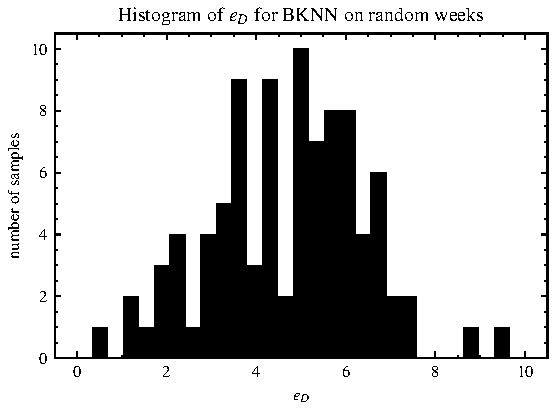
\includegraphics[width=\textwidth]{chapters/figures/result_histograms/result_histogram_random_week_workload_dist_error_BKNN.pdf}
%         \captionsetup{width=.9\linewidth}
%         \caption{}
%     \end{subfigure}%
%     ~ 
%     \begin{subfigure}[t]{0.45\textwidth}
%         \centering
%         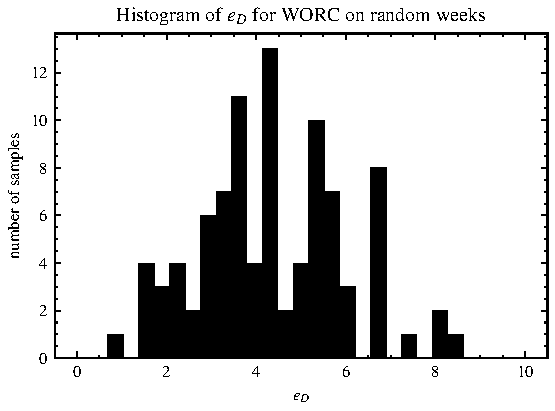
\includegraphics[width=\textwidth]{chapters/figures/result_histograms/result_histogram_random_week_workload_dist_error_WORC.pdf}
%         \captionsetup{width=.9\linewidth}
%         \caption{}
%     \end{subfigure}
%     \\[1ex]
%     \centering
%     \begin{subfigure}[t]{0.45\textwidth}
%         \centering
%         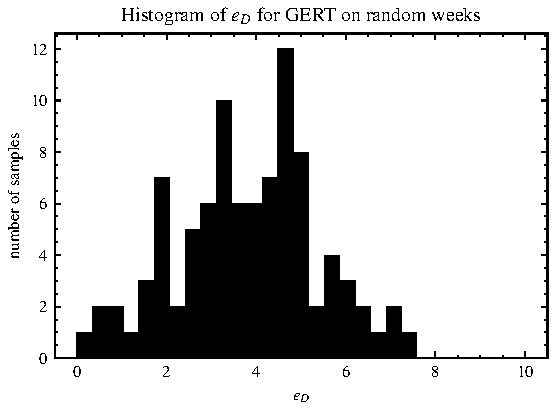
\includegraphics[width=\textwidth]{chapters/figures/result_histograms/result_histogram_random_week_workload_dist_error_GERT.pdf}
%         \captionsetup{width=.9\linewidth}
%         \caption{}
%     \end{subfigure}%
%     ~ 
%     \begin{subfigure}[t]{0.45\textwidth}
%         \centering
%         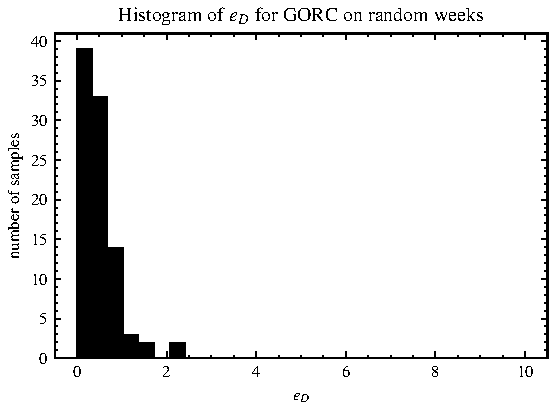
\includegraphics[width=\textwidth]{chapters/figures/result_histograms/result_histogram_random_week_workload_dist_error_GORC.pdf}
%         \captionsetup{width=.9\linewidth}
%         \caption{}
%     \end{subfigure}
%     \caption{Histogram of distribution error for the different models on the random weeks data set}
%     \label{fig:result_random_week_dist}
% \end{figure}

% \begin{figure}[t]
%     \centering
%     \begin{subfigure}[t]{0.45\textwidth}
%         \centering
%         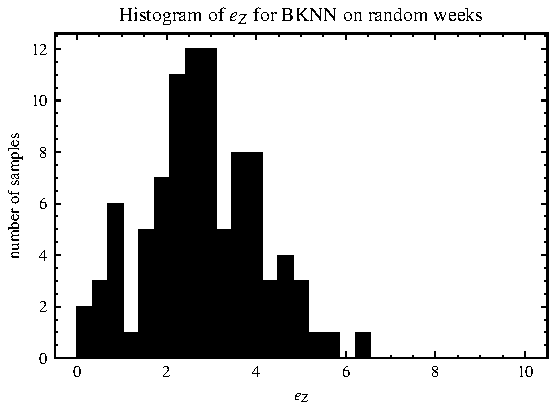
\includegraphics[width=\textwidth]{chapters/figures/result_histograms/result_histogram_random_week_zone_sum_error_BKNN.pdf}
%         \captionsetup{width=.9\linewidth}
%         \caption{}
%     \end{subfigure}%
%     ~ 
%     \begin{subfigure}[t]{0.45\textwidth}
%         \centering
%         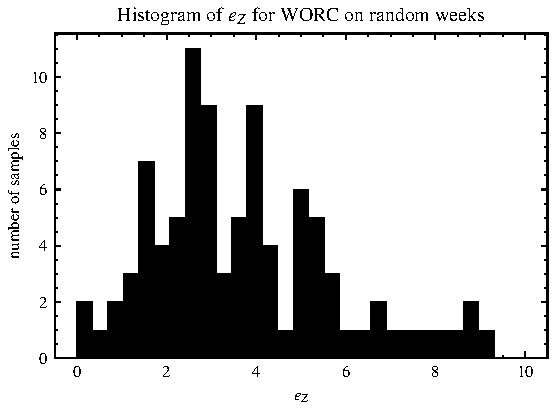
\includegraphics[width=\textwidth]{chapters/figures/result_histograms/result_histogram_random_week_zone_sum_error_WORC.pdf}
%         \captionsetup{width=.9\linewidth}
%         \caption{}
%     \end{subfigure}
%     \\[1ex]
%     \centering
%     \begin{subfigure}[t]{0.45\textwidth}
%         \centering
%         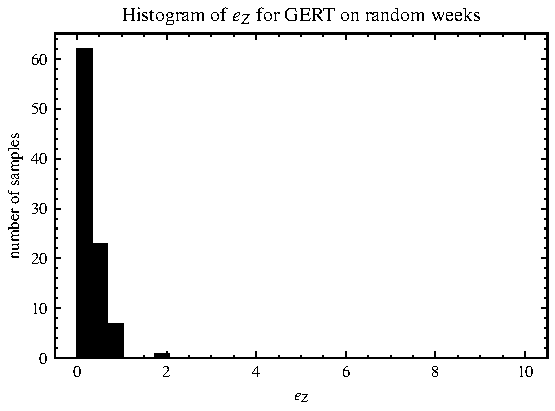
\includegraphics[width=\textwidth]{chapters/figures/result_histograms/result_histogram_random_week_zone_sum_error_GERT.pdf}
%         \captionsetup{width=.9\linewidth}
%         \caption{}
%     \end{subfigure}%
%     ~ 
%     \begin{subfigure}[t]{0.45\textwidth}
%         \centering
%         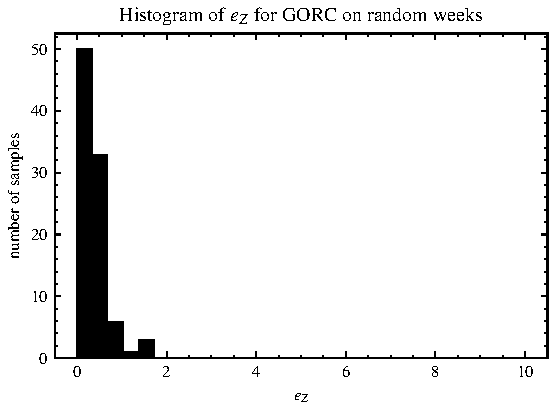
\includegraphics[width=\textwidth]{chapters/figures/result_histograms/result_histogram_random_week_zone_sum_error_GORC.pdf}
%         \captionsetup{width=.9\linewidth}
%         \caption{}
%     \end{subfigure}
%     \caption{Histogram of zone error for the different models on the random splits data set}
%     \label{fig:result_random_week_zones}
% \end{figure}

In \cref{fig:preds}, the total training load decided by the Baseline KNN model and GERT respectively are plotted against the total training load decided by the coach for all training plans in the test set \textit{random weeks}.
From the figures, it is clear that the Baseline KNN model, even though it does a decent job of mimicking the coach's total training load, is outperformed by the GERT model, which does a near-perfect job mimicking the coach's total training load.

\begin{figure}[t]
    \centering
    \begin{subfigure}{0.45\textwidth}
        \centering
        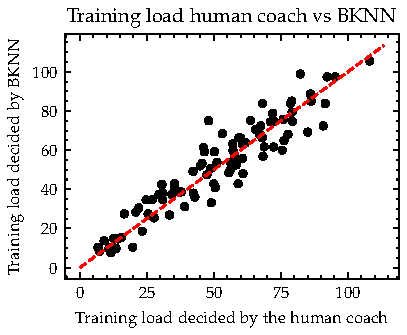
\includegraphics[width=0.9\textwidth]{chapters/figures/result/result_total_load_BKNN_vs_coach.pdf}
        \captionsetup{width=.9\linewidth}
        \caption{Training load of a weekly program set by the human coach versus that training program automatically generated by BKNN for all data points in the held-out test set. The dashed red line highlights the target function of perfect correspondence.}
        \label{subfig:BKNN_pred}
    \end{subfigure}
    \begin{subfigure}{0.45\textwidth}
        \centering
        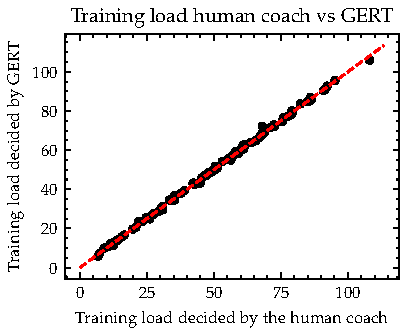
\includegraphics[width=0.9\textwidth]{chapters/figures/result/result_total_load_GERT_vs_coach.pdf}
        \captionsetup{width=.9\linewidth}
        \caption{Training load of a weekly program set by the human coach versus that training program automatically generated by GERT for all data points in the held-out test set. The dashed red line highlights the target function of perfect correspondence.}
        \label{subfig:GERT_pred}
    \end{subfigure}
    \caption{Comparison of how well the two models Baseline KNN (BKNN) and GERT can mimic the total training load set by the human coach.
    }
    \label{fig:preds}
\end{figure}

Another aspect of the GERT model is the time it takes to create a training plan.
When producing the results GERT took on average \SI{1.4}{\second} to generate a weekly plan on an ordinary workstation.\footnote{Intel\textregistered{} Core\texttrademark{} i7-3770 CPU @ 3.40GHz - 3 cores}

Next, some examples of outputs from the GERT model are presented.
An example of a good output is presented in \cref{fig:gert_good_example}.
The training plan generated by GERT follows a similar structure to that of a human coach in terms of training load distribution over the week, session types and intensity zone distribution.
The two training plans only differ slightly in order of the session types, as can be seen in the morning sessions of the later sessions of the week.
% Further, the training plan by the human coach is structured in such a way that the high intensity sessions are put on days where only one session is performed, while the days with double sessions have lower intensity sessions.

\begin{figure}[ht]
    \centering
    \begin{subfigure}[t]{0.7\textwidth}
        \centering
        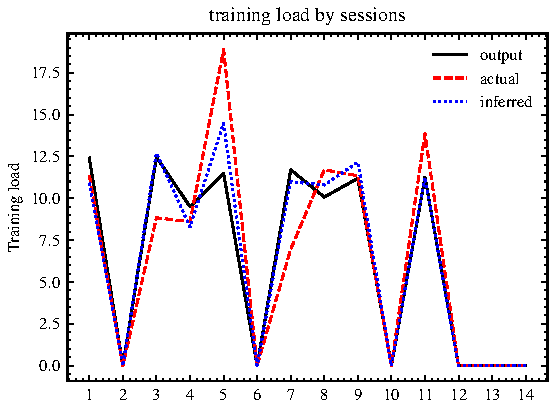
\includegraphics[width=\textwidth]{chapters/figures/result_examples/good_dist.pdf}
        \captionsetup{width=.9\linewidth}
        \caption{The distribution of training load over the sessions of the week for the plan that was generated by GERT (output), the distribution that was predicted by GERT's regressor (inferred), and the distribution of the week written by the human coach (actual).}
    \end{subfigure}%

    \begin{subfigure}[t]{0.7\textwidth}
        \centering
        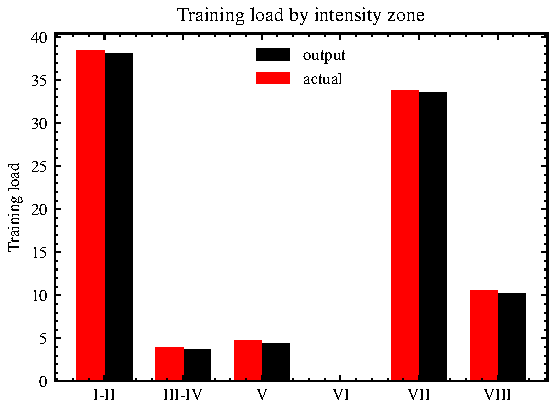
\includegraphics[width=\textwidth]{chapters/figures/result_examples/good_zone.pdf}
        \captionsetup{width=.9\linewidth}
        \caption{The distribution of training load over the intensity zones of the week for the plan that was generated by GERT (output) and the human coach (actual).}
    \end{subfigure}
    \caption{An example of where GERT succeeded in generating a training plan similar to the human coach.}
\end{figure}
\begin{figure}\ContinuedFloat
    \begin{subfigure}[t]{\textwidth}
        \centering
        
\includegraphics[width=\textwidth,trim={0 8cm 0 0},clip]{chapters/figures/result_examples/good_pred.pdf}
        \captionsetup{width=.9\linewidth}
        \caption{The training plan generated by GERT.}
    \end{subfigure}
    
    \begin{subfigure}[t]{\textwidth}
        \centering
        
\includegraphics[width=\textwidth,trim={0 8cm 0 0},clip]{chapters/figures/result_examples/good_true.pdf}
        \captionsetup{width=.9\linewidth}
        \caption{The training plan from the human coach.}
    \end{subfigure}
    \caption{(cont.) An example of where GERT succeeded in generating a training plan similar to the human coach.}
    \label{fig:gert_good_example}
\end{figure}

\cref{fig:gert_bad_example} shows an example where GERT's training plan scored worse than average.
Although both weeks contain the same number and types of sessions, the sessions are performed on different days compared to those of the human coach. 
As can be seen in the \cref{fig:gert_bad_example_distribution} GERT tries to adapt the sessions to the inferred distribution, which is different from the actual distribution.
Note how the inferred training load distribution, even though erroneous, more closely resembles the actual distribution compared to the generated training plan.
Note also that the actual training plan includes two new triplets of session types, (anc, aec23, aep) and (aec23, aep, rest), not present in the training data, that GERT is discouraged from using.

\begin{figure}[ht]
    \centering
    \begin{subfigure}[t]{0.7\textwidth}
        \centering
        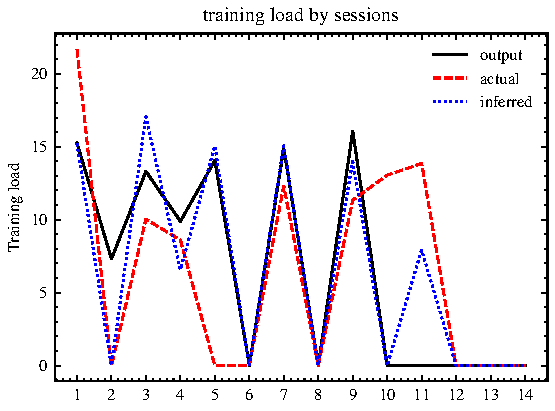
\includegraphics[width=\textwidth]{chapters/figures/result_examples/bad_dist.pdf}
        \captionsetup{width=.9\linewidth}
        \caption{The distribution of training load over the sessions of the week for the plan that was generated by GERT (output), the distribution that was predicted by GERT's regressor (inferred), and the distribution of the week written by the human coach (actual).}
        \label{fig:gert_bad_example_distribution}
    \end{subfigure}

    \begin{subfigure}[t]{0.7\textwidth}
        \centering
        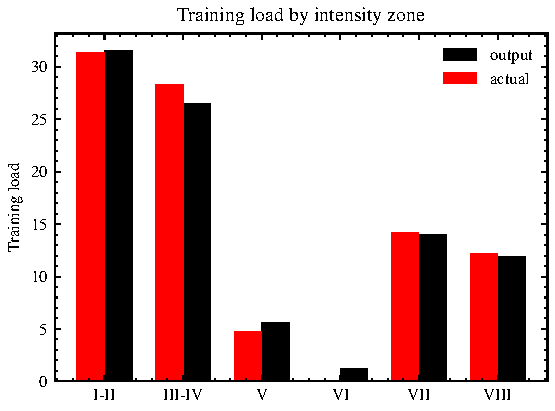
\includegraphics[width=\textwidth]{chapters/figures/result_examples/bad_zone.pdf}
        \captionsetup{width=.9\linewidth}
        \caption{The distribution of training load over the intensity zones of the week for the plan that was generated by GERT (output) and the human coach (actual).}
    \end{subfigure}
    \caption{An example of where GERT failed to generate a training plan similar to the human coach. Note how the generated plan has sessions on Monday afternoon and Wednesday morning, while the actual plan has sessions on Friday afternoon and Saturday morning.}
\end{figure}
\begin{figure}\ContinuedFloat
    \begin{subfigure}[t]{\textwidth}
        \centering
        
\includegraphics[width=\textwidth,trim={0 8cm 0 0},clip]{chapters/figures/result_examples/bad_pred.pdf}
        \captionsetup{width=.9\linewidth}
        \caption{The training plan generated by GERT.}
    \end{subfigure}
    
    \begin{subfigure}[t]{\textwidth}
        \centering
        
\includegraphics[width=\textwidth,trim={0 8cm 0 0},clip]{chapters/figures/result_examples/bad_true.pdf}
        \captionsetup{width=.9\linewidth}
        \caption{The training plan from the human coach.}
    \end{subfigure}
    \caption{(cont.) An example of where GERT failed to generate a training plan similar to the human coach. Note how the generated plan has sessions on Monday afternoon and Wednesday morning, while the actual plan has sessions on Friday afternoon and Saturday morning.}
    \label{fig:gert_bad_example}
\end{figure}

An example of one of GERT's worst scoring plans can be seen in \cref{fig:gert_worst_example}.
Here, the sessions of the week are put in the completely wrong days, resulting in a very large distribution error.
Although the distribution is off compared to the human plan, note that both sessions are planned for two consecutive days, similar to the human coach, but on the wrong days.

\begin{figure}[ht]
    \centering
    \begin{subfigure}[t]{0.7\textwidth}
        \centering
        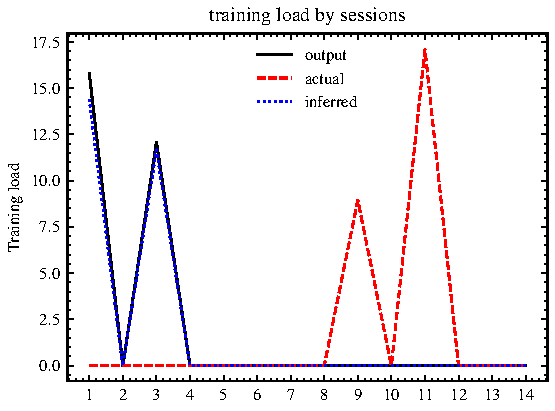
\includegraphics[width=\textwidth]{chapters/figures/result_examples/worst_dist.pdf}
        \captionsetup{width=.9\linewidth}
        \caption{The distribution of training load over the sessions of the week for the plan that was generated by GERT (output), the distribution that was predicted by GERT's regressor (inferred), and the distribution of the week written by the human coach (actual).}
    \end{subfigure}%

    \begin{subfigure}[t]{0.7\textwidth}
        \centering
        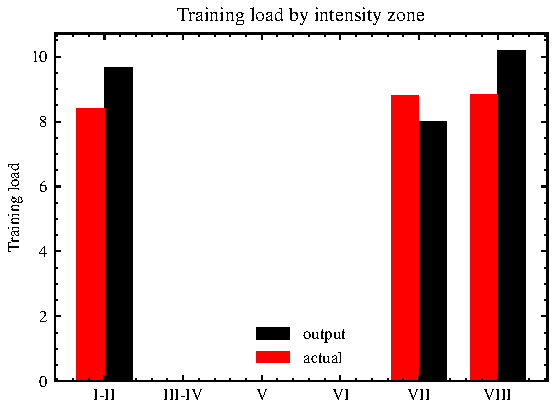
\includegraphics[width=\textwidth]{chapters/figures/result_examples/worst_zone.pdf}
        \captionsetup{width=.9\linewidth}
        \caption{The distribution of training load over the intensity zones of the week for the plan that was generated by GERT (output) and the human coach (actual).}
    \end{subfigure}
    \caption{An example of a sparse training week where GERT generated a training plan that was scored as very different to the human coach.}
\end{figure}
\begin{figure}\ContinuedFloat
    \begin{subfigure}[t]{\textwidth}
        \centering
        
\includegraphics[width=\textwidth,trim={0 8cm 0 0},clip]{chapters/figures/result_examples/worst_pred.pdf}
        \captionsetup{width=.9\linewidth}
        \caption{The training plan generated by GERT.}
    \end{subfigure}\\[1ex]
    \begin{subfigure}[t]{\textwidth}
        \centering
        
\includegraphics[width=\textwidth,trim={0 8cm 0 0},clip]{chapters/figures/result_examples/worst_true.pdf}
        \captionsetup{width=.9\linewidth}
        \caption{The training plan from the human coach.}
    \end{subfigure}
    \caption{(cont.) An example of a sparse training week where GERT generated a training plan that was scored as very different to the human coach.}
    \label{fig:gert_worst_example}
\end{figure}

\FloatBarrier
\section{Discussion}

In this section, the result seen in the previous section will be discussed.
We also highlight differences between models that, to different extents, generate new training plans and those that find complete plans.
Some of the more important assumptions that have been made are also discussed as well as their effects if they are false.
Lastly, some shortcomings of the data set, some metrics, and GERT are discussed together with a few possible improvements.

\subsection{Discussion of Results}

From the results in \cref{tab:results}, it is clear that the distribution of training load over the sessions, $e_D$, was difficult for the non-oracle models to minimize.
This is expected since the information is not explicitly given in the input.
The small difference between the weekly oracle model and the Baseline KNN model on that same metric show that a model based on picking complete training plans would not perform significantly better, on this data set, even if it could estimate the target perfectly.
The large difference between the GERT and GERT Oracle for the $e_D$ error shows the biggest shortcoming of GERT, which is the weekly distribution.
GERT's estimation of the target for $e_D$ is the only difference between the models and must therefore be responsible for the performance difference.

% From the results in \cref{tab:results}, it can also be seen that the Baseline KNN model performs significantly better on the $e_Z$ metric compared to the Weekly Oracle model.
% The reason for this is almost certainly the construction of the Baseline KNN model.
% Since this model tries to find the weekly plan corresponding to the input most similar to the queried input, and because the input contain the training load distribution over the intensity zones, the Baseline KNN model will, as a side effect, minimize this metric.
% The Baseline KNN model knows noting about the metrics or loss function, it will therefore not balance the minimization of $e_Z$ against the other metrics in the same way that the other models, especially the Weekly error, would.
% This results in the Baseline being able to outperform the Weekly Oracle model on this single metric, but has a much higher score on the total loss function.


There might be a difference in performance between the three ways of splitting the data set into train and test sets seen in \cref{tab:results}, but the difference is not significant.
If there is a difference it is likely the result of two different aspects.
The first being that, when splitting so that the chronologically last data makes up the test set, the test set is fully composed of data gathered during the COVID-19 pandemic.
It is reasonable to believe that the unusual circumstances of the time, with restrictions on travel, social interaction, and canceled competitions, have resulted in training plans which are different from those created during a time without the pandemic.
Selecting a large fraction of the data points from the pandemic time period and creating a test set of the same will result in a distributional shift in the test set.
This makes the planning task an out of distribution prediction which is significantly more difficult.
The fact that the performance difference is not bigger can probably be accounted for by the training set still containing a sufficiently large number of data points from the pandemic, and that the input to the model contains information for some of the targets for the metrics.
Support for this hypothesis should be seen as the weekly distribution score, $e_D$, for GERT being more affected than the zone distribution score, $e_Z$. 
Since $e_D$ is estimated from historical data, while $e_Z$ is given in \textit{weekly input}, a distributional shift due to the pandemic would affect $e_D$ more.
The results might be slightly indicative of this but the effect is not significant and can be the effect of random noise.

The second aspect to the possible difference in performance for the three ways of splitting is that the athletes often train together.
Similar athletes are often assigned similar training plans.
When performing the split that randomly assigns data points to the train and test set, some of the similar training plans can end up in each of the data sets.
See \cref{fig:random_splits} for an illustration of the splitting algorithm.
This gives the models the slight advantage of having seen a similar case before and can therefore create a queried training plan that is more accurate.
For this hypothesis to hold, there should be minimal to no effect seen for the genetic algorithm module of the GERT model, but an impact on the estimation of the distribution of training load over the sessions.
That is, the $e_D$ score would be affected between the \textit{random sample} and \textit{random weeks} while the $e_Z$ score was not.
This effect might be present in the \cref{tab:results} but the possible difference in $e_D$ is not significant and could be attributed to random noise.
Hence, we can not conclude, from our data, that the different splits had a significant impact on the results of the experiments.

\Cref{fig:gert_good_example,fig:gert_bad_example,fig:gert_worst_example} display many interesting aspects of how GERT produces its training plans.
It is clear that the inferred training load distribution is the source of much of the error, but it must also be noted that the produced training plan sometimes has training load distributions that deviate from the inferred one as well.
Three reasons that could result in this behavior.
First, this could be a result of early stopping.
Since the genetic algorithm optimization results in a stochastic search of the output space, it is improbable that the globally optimal result will be found in any feasible amount of time.
The longer GERT runs the better the produced training plans should be.
Because of this trade-off between run time and performance, it is plausible that the search has not properly converged yet when the termination criterion is triggered.
This could in turn be because that the algorithm got stuck in a local minimum, or that the rate of improvement plateaued.

The second reason why the training load distributions of the produced training plan might deviate from the inferred is because of an interplay between the different metrics in the loss function.
An example of this can be seen in \cref{fig:gert_bad_example}.
Even though the regressor predicts that there should be a rest session on Monday afternoon, the genetic algorithm part of the algorithm fails to follow the inferred distribution.
The reason for this behavior is that the plan from the human coach contains two new triplets that have not been present in \textit{detailed plans}$_{test}$, \textit{(anc, aec23, aep)} and \textit{(aec23, aep, rest)}.
Since the penalty for deviating from the triplets was set higher than deviating from the distribution of training load over sessions, GERT tries to create a plan that only contains known triplets.

The third reason is that there might not exist a perfect solution.
It is entirely possible, and even probable, that, given the relatively small training data set, there exist some targets that can not be fulfilled all at the same time by a training plan created from the sessions in the training data set.
In such a case, GERT will produce a training plan that is as close as possible to fulfilling the targets, while balancing the errors in accordance with the weights on the metrics in the loss function.

\subsection{Model basis}
The results show big advantages of being able to create a training plan by selecting sessions rather than having to select a complete week.
The Weekly Oracle model, which selects the complete week that would give the best scores knowing the output, is outperformed by GERT, which selects sessions to build a new training plan, on all scores.
This is without a doubt because of the added flexibility of GERT, letting it customize a training plan to minimize all scores.
It is this same high level of flexibility that lets GERT mimic the total training load set by the coach in a way that the Baseline KNN model can not, see \cref{fig:preds}.

Another advantage of using a model that creates new plans from a session library rather than selecting historic plans is the possibility of constructing out of distribution plans.
If a model based on selecting historical weeks is queried for a training plan which is significantly different from what it is trained on, the model's only option is to return a plan that does not fit the requirements.
This is not necessarily the case for a model that creates its train plans from a session library.
This model can in some cases construct a new plan that fulfills the requirements even though none of the plans it has trained on has done so.

The previous two paragraphs have both looked at the differences between the ways of creating training plans from the perspective of a limited data setting, which is the case for this work, but there is also another, more fundamental, aspect to it.
There exists a trade-off between creating training plans of guaranteed quality, but where the set of possible output plans are rigid and dependent on the training data, versus creating training plans where the flexibility and versatility of the produced plans are much higher.
In this thesis we have only included two points of this range, returning complete historical plans which are known to be good, or returning plans based on individual sessions which you also have to make sure work together.
Other options include, but are not limited to, creating training plans based on larger groups of sessions, making the plans more rigid but making quality plans easier to produce; or creating plans based on individual exercises, making it possible to create unique training plans but making the problem of quality immensely difficult.
The preferred trade-off varies between problem settings.
For the case with limited data, where the use case for the model is out of distribution, or when quality is none critical, a more flexible solution is arguably the better option.
On the other hand, if the quality is crucial and the model will be used for similar cases that it has been trained on, a more rigid model might be preferred. 

\subsection{Assumptions}
During this work, the assumption has been made that the training in the data set reported by the athletes is the same as the training the coach planned for.
There are two different scenarios we see where this assumption would not hold.
The first one is when the coach makes adjustments to the plan as a response to an unforeseen event.
For example, the athlete might feel under the weather and need a lighter training load, the athlete might have been injured and is unable to perform the originally planned training, or the athlete might be more recovered than what was expected and require a heavier training load.
In all these cases the cause of the adjustment could not have been predicted based on the features provided to the model.
The consequences of this are that these alterations appear as noise to the model.
As long as the alterations are unstructured and do not make up a large portion of the data set, GERT should still be able to learn the way the coach produces the training plans.
However, if the alterations follow an underlying structure it is likely that GERT develops a bias and starts to plan not as the coach originally would have done, but instead tries to include the alterations in its plans.
The effects of this assumption are hard to investigate without a complete data set of the coach's original planning, although it is reasonable to believe that most of the training happened according to plan.

The second way that the assumption can break is if the athlete does not report the training accurately.
There may be a discrepancy between the training reported by the athletes and what was performed.
This means that even if the athletes performed the training prescribed by the coach, it is not certain that the session was reported correctly.
This would be similar to the first case in terms of effect.
If the effect is random, such as if the athlete miscounts the number of repetitions, GERT should still be able to learn how the coach makes the plans.
If the effect is systematic, for example, if the athletes always skip the last repetition, then GERT will probably pick up a bias and instead produce training plans that the athletes are likely to report doing rather than what the coach plans.
During conversations with the coach, it was pointed out that some athletes are better at reporting their training than others, and that some athletes are better at reporting when they are performing well or are training for a competition compared to when they are underperforming or are in the off-season.
This issue is likely further enhanced by the pandemic since many competitions have been cancelled.
These types of discrepancies in the reporting is a systematic error and would, as described above, likely lead to a bias.
This is, similarly to the first issue, hard to investigate without additional data.

During this work, we also make the assumption that the weekly plans are independent of each other given the macro- and mesoplans.
This allows for the problem of creating the weekly plans to be approached on a week by week basis, without the need for the complexity of creating dependent plans.
If the assumption is not true, the contents and order of the sessions would be wrongly predicted, since they are not specified in the meso- or macroplan.
This would result in an increased $e_D$ score.
This may be the cause for at least some of the increase in $e_D$ score observed between GERT and GERT Oracle since the GERT Oracle utilizes the true weekly training load distribution.
It is difficult to investigate whether or not this assumption holds because the alternatives for how the plans are connected are infinite and have to be compared to find the one with the best predictive power.
One alternative is to let the coach describe the connections, but this assumes that the coach is aware of the connections and can formulate them as stringent rules.

\subsection{Shortcomings}
Based on the comparison between the GERT and GERT Oracle we can see both that the genetic planner is good at adapting a plan to a given distribution and that the inferred distribution is not always correct.
GERT could therefore be improved upon by improving the inferred weekly distribution.
However, some of the cases that are inferred erroneously by the GERT might be less erroneous than the metrics indicate.

Consider the case when an athlete only trains one session during the whole week.
From a physiological standpoint, it should not be a difference between having that session on a Wednesday morning compared to on a Thursday morning.
The $e_D$ metric would however consider this is an error and score it accordingly.
Since similar cases occur multiple times, located differently in the week, the regressor inferring the training load distribution has no way of knowing where to place the training load this time.
What is missing is some sense of time invariance.
After some number of contiguous rest sessions, adding another one will not make a difference for the quality of the training.
Although the length of this sequence would need to be investigated, we present an example where the sequence length is 3.
The earlier example with one session performed on Wednesday morning can then be seen as three or more \textit{rest}, followed by a session, followed by three or more \textit{rest}.
The same is true for performing one session on Thursday, and the two weeks can now be considered equivalent.
Using such a construction when evaluating GERT would decrease the reported $e_D$ score for some of the cases and also result in scores that might more closely match the physiological notion of equivalence.

The previously discussed error is not the only one that occurs.
As comparing the results from GERT and GERT Oracle indicate, it is possible to greatly improve GERT's results by improving the weekly distribution.
This is very interesting from a practitioner's perspective since there is nothing that stops the user from specifying the training load input on a daily basis rather than a weekly.
For example, it would be possible to combine GERT with the work of Kumayito~\cite{kumyaito2018planning}, who uses Adaptive PSO to find an optimal training load per day for an entire macro-plan.
This would create a pipeline where an optimal daily training load was calculated based on parameters from the Busso model~\cite{busso2006using}, the coach could then specify the main sets for the week and GERT would create a training plan for the athlete.

The data set that we have worked with have in many ways been limiting.
First of all, the data set only contains data for a single coach.
This means that we have no way of investigating the generalizability of our model, GERT, to other coaches or athletes with other coaches.
Next, all athletes in the data set are elite athletes.
This limits our ability to test the generalizability of GERT to other classes of athletes such as hobbyists or junior elites.
We have also only focused on swimming, as this is what we have data on.
We will, despite this, try to reason about GERT and try to understand its potential.

While building GERT we made assumptions that were specific to our data, such as the number of sessions per week and types of sessions.
These assumptions have, among other things, affected the metrics in the loss function and the structure of sessions in a micro plan.
However, the main idea of creating training plans from a session library by using a genetic algorithm is in no way specific to the investigated coach or our data and should, with some small amount of adaptation, be able to generalize to other coaches and athletes than those found on our data set. 
By the same reasoning, similar constructions can be made for most other endurance sports.
This leads us to believe that our implementation of GERT could be easily adapted to successfully create plans for many other sports. 

It is important to note that our evaluation of the training plans is completely quantitative.
Qualitative aspects of the plans are ignored.
We also only have a relatively small feature set to work with.
There might be aspects to the training plans that can not be fully or at all captured by the features that we used.
This would imply that our metrics and loss function are incomplete.
It would be naive to think that the current metrics capture the entire spectra and knowledge that goes into building a training plan.
For example, we do not take the full contents of the training sessions into consideration.
Although we perform well in terms of the model goals and metrics specified, this work is a first step and could be extended indefinitely to capture more aspects of the task.
